
\section{ Check CBF SKARAB Health}

Simply follow the link to see CBF overall health\\ \url{http://cbf-nuc2.cpt.kat.ac.za/cmc1/array\_1.wide} or \url{http://mon-cbf.kat.ac.za/}

\section{ MeerKAT Status Sensor Summary}
This too is a swift troubleshooting tool querying essential observation sensors from all active APs thus cutting down a systematic fault-finding approach.   

Log onto the obs mkat machine and run the script below and the output will appear  as shown in \textbf{Figure}~\ref{fig:image78} for L-band or \textbf{Figure}~\ref{fig:image107} for U-band:
\begin{lstlisting}[style=DOS]
ssh kat@obs.mkat.karoo.kat.ac.za
python usersnfs/tiyani/meerkat\_status.py --receiver-band rxl --send-status   

\end{lstlisting}


\begin{figure}[!thb]
	\centering
	%\includegraphicsdpi{100}{}{bur1.png}     
	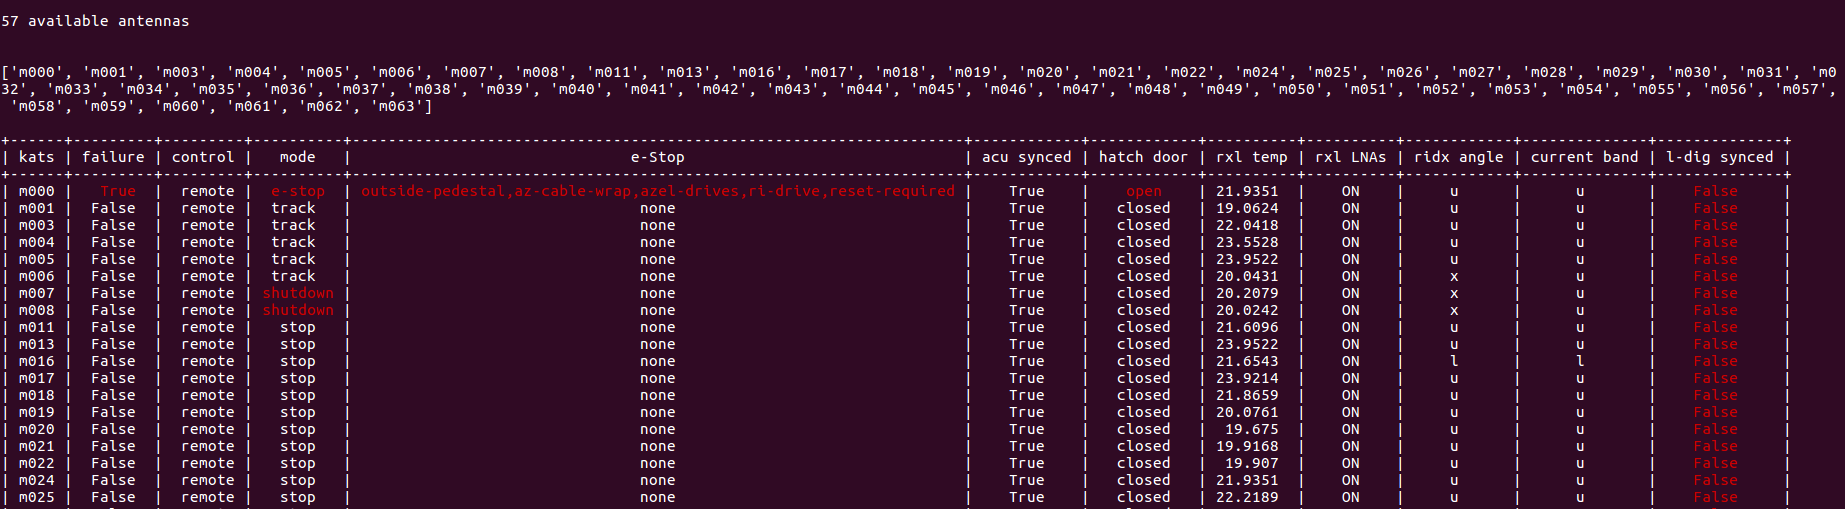
\includegraphics[scale=0.18]{Chapters/images/image78.png}
	
	%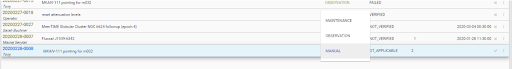
\includegraphics[resolution=100]{bur1.png}
	\caption{Meerkat status script  output for U-band}
	\label{fig:image78}
\end{figure}



\begin{figure}[!thb]
	\centering
	%\includegraphicsdpi{100}{}{bur1.png}     
	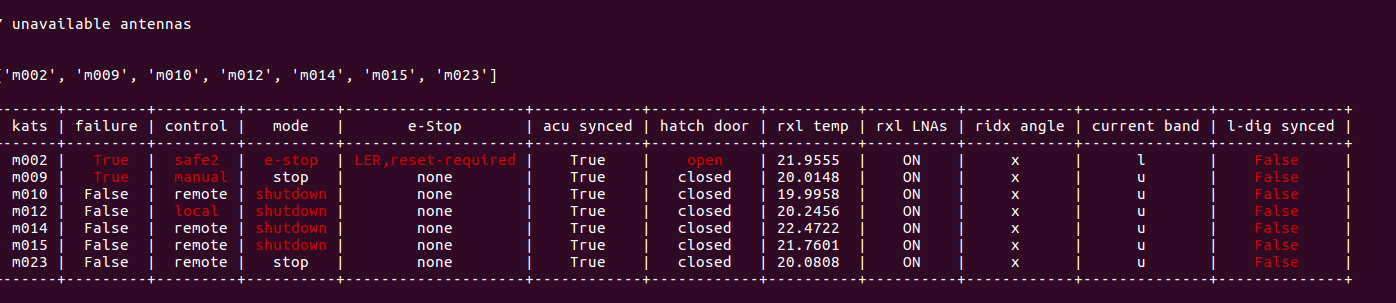
\includegraphics[scale=0.23]{Chapters/images/image107.png}
	
	%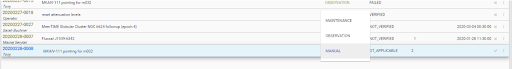
\includegraphics[resolution=100]{bur1.png}
	\caption{Meerkat status script  output for L-band}
	\label{fig:image107}
\end{figure}

         




\section{ Monitor an active observation}
\subsection{Catalogues Not Matching The Observation}
If and when this happens, contact the AoD. Best practice to avoid it is by running a dryrun while there are still astronomers in the office

Once the observation begins,monitor the following for “no descriptor” errors:
\begin{itemize}

\item \textbf{no-descriptor}-heaps-total for each band on the sdp\_1 GUI sensor list. 
\item Go to the GUI, select sensor list and then select sdp\_1.
\item There are four ingest nodes where each has ¼ of the band.
\item Search for “desc” and hide nominals, the no-descriptor-heaps--total should preferably remain at zero for all ingest nodes (see \textbf{Figure}~\ref{fig:image129}) but there are times where one or two ingest nodes will increase for a very short period after the observation begins.

\begin{figure}[!thb]
	\centering
	%\includegraphicsdpi{100}{}{bur1.png}     
	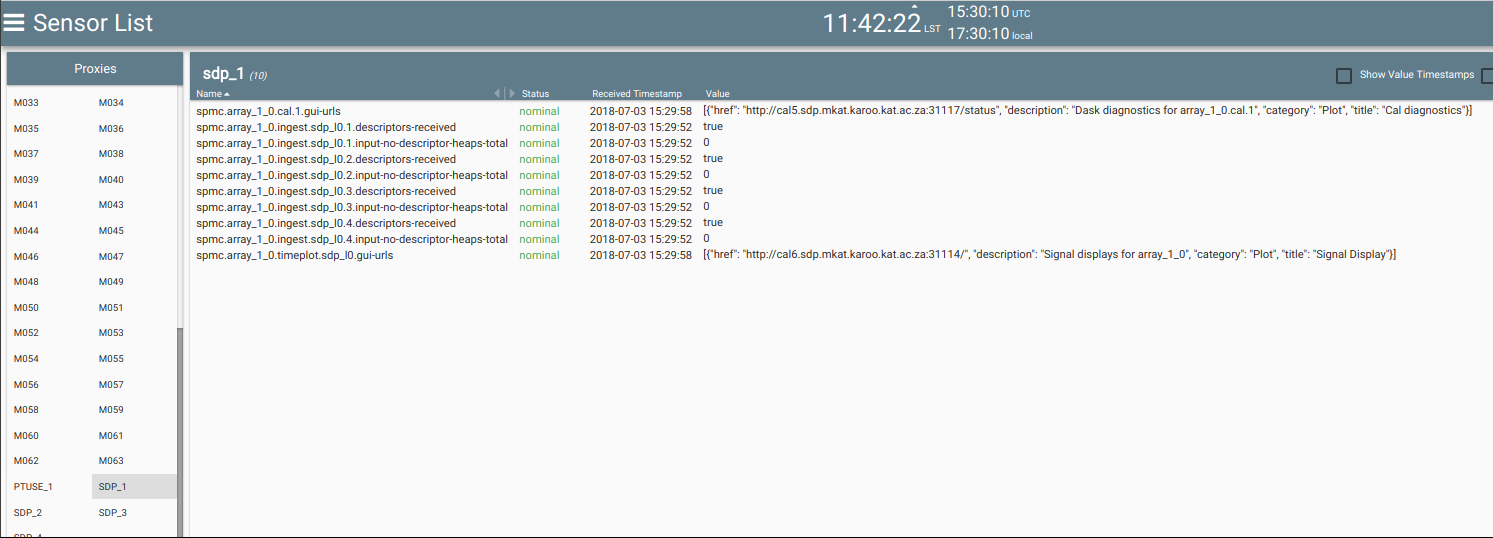
\includegraphics[scale=0.26]{Chapters/images/image129.png}
	
	%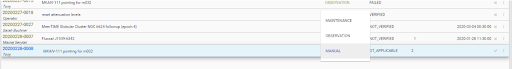
\includegraphics[resolution=100]{bur1.png}
	\caption{SDP sensors}
	\label{fig:image129}
\end{figure}
\item This is okay, as long as they all do not keep increasing to very high numbers.If this happens then break down the subarray, reload the Mellanox switch and rebuild the array.
	




\item SDP Grafana GUI interface, this can be accessed via 	\url{http://mc1.sdp.mkat.karoo.kat.ac.za:3000/?orgId=1}  Select the "\textbf{Overview}" option. 

\item There are other options which are available from the dashboard as shown in \textbf{Figure}~\ref{fig:image11}.

\begin{figure}[H]
	\centering
	%\includegraphicsdpi{100}{}{bur1.png}     
	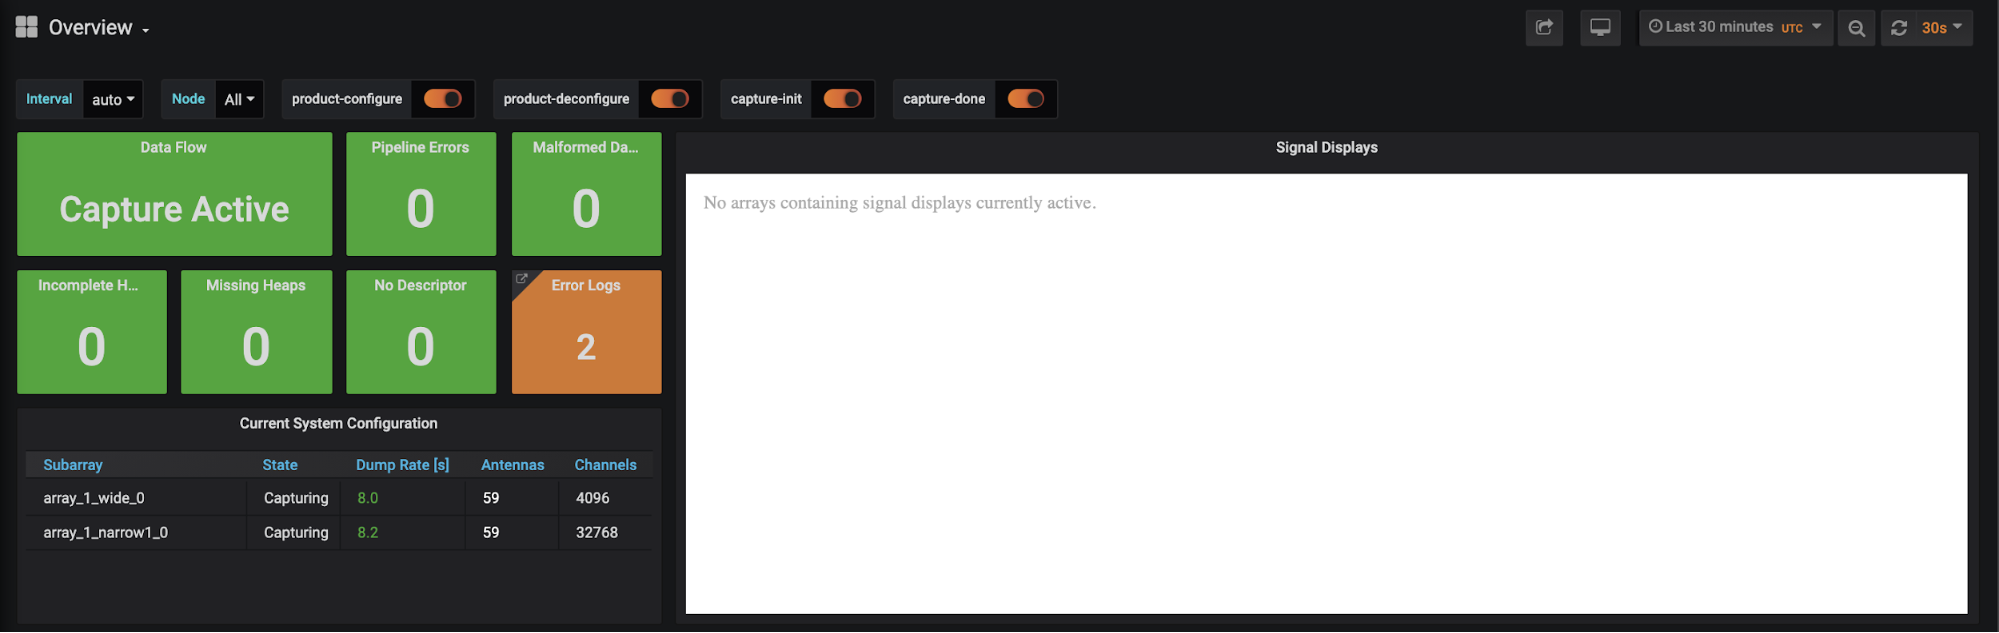
\includegraphics[scale=0.22]{Chapters/images/image11.png}
	
	%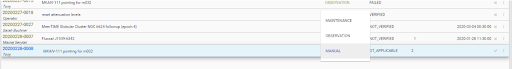
\includegraphics[resolution=100]{bur1.png}
	\caption{SDP Grafana dashboard}
	\label{fig:image11}
\end{figure}


When running the observation, the dashboard will most likely show “no descriptor” errors at the beginning of the observation.  No descriptor block and/or incomplete heaps block are orange, these values should return to zero within five minutes as shown in \textbf{Figure}~\ref{fig:image15}.

\begin{figure}[!thb]
	\centering
	%\includegraphicsdpi{100}{}{bur1.png}     
	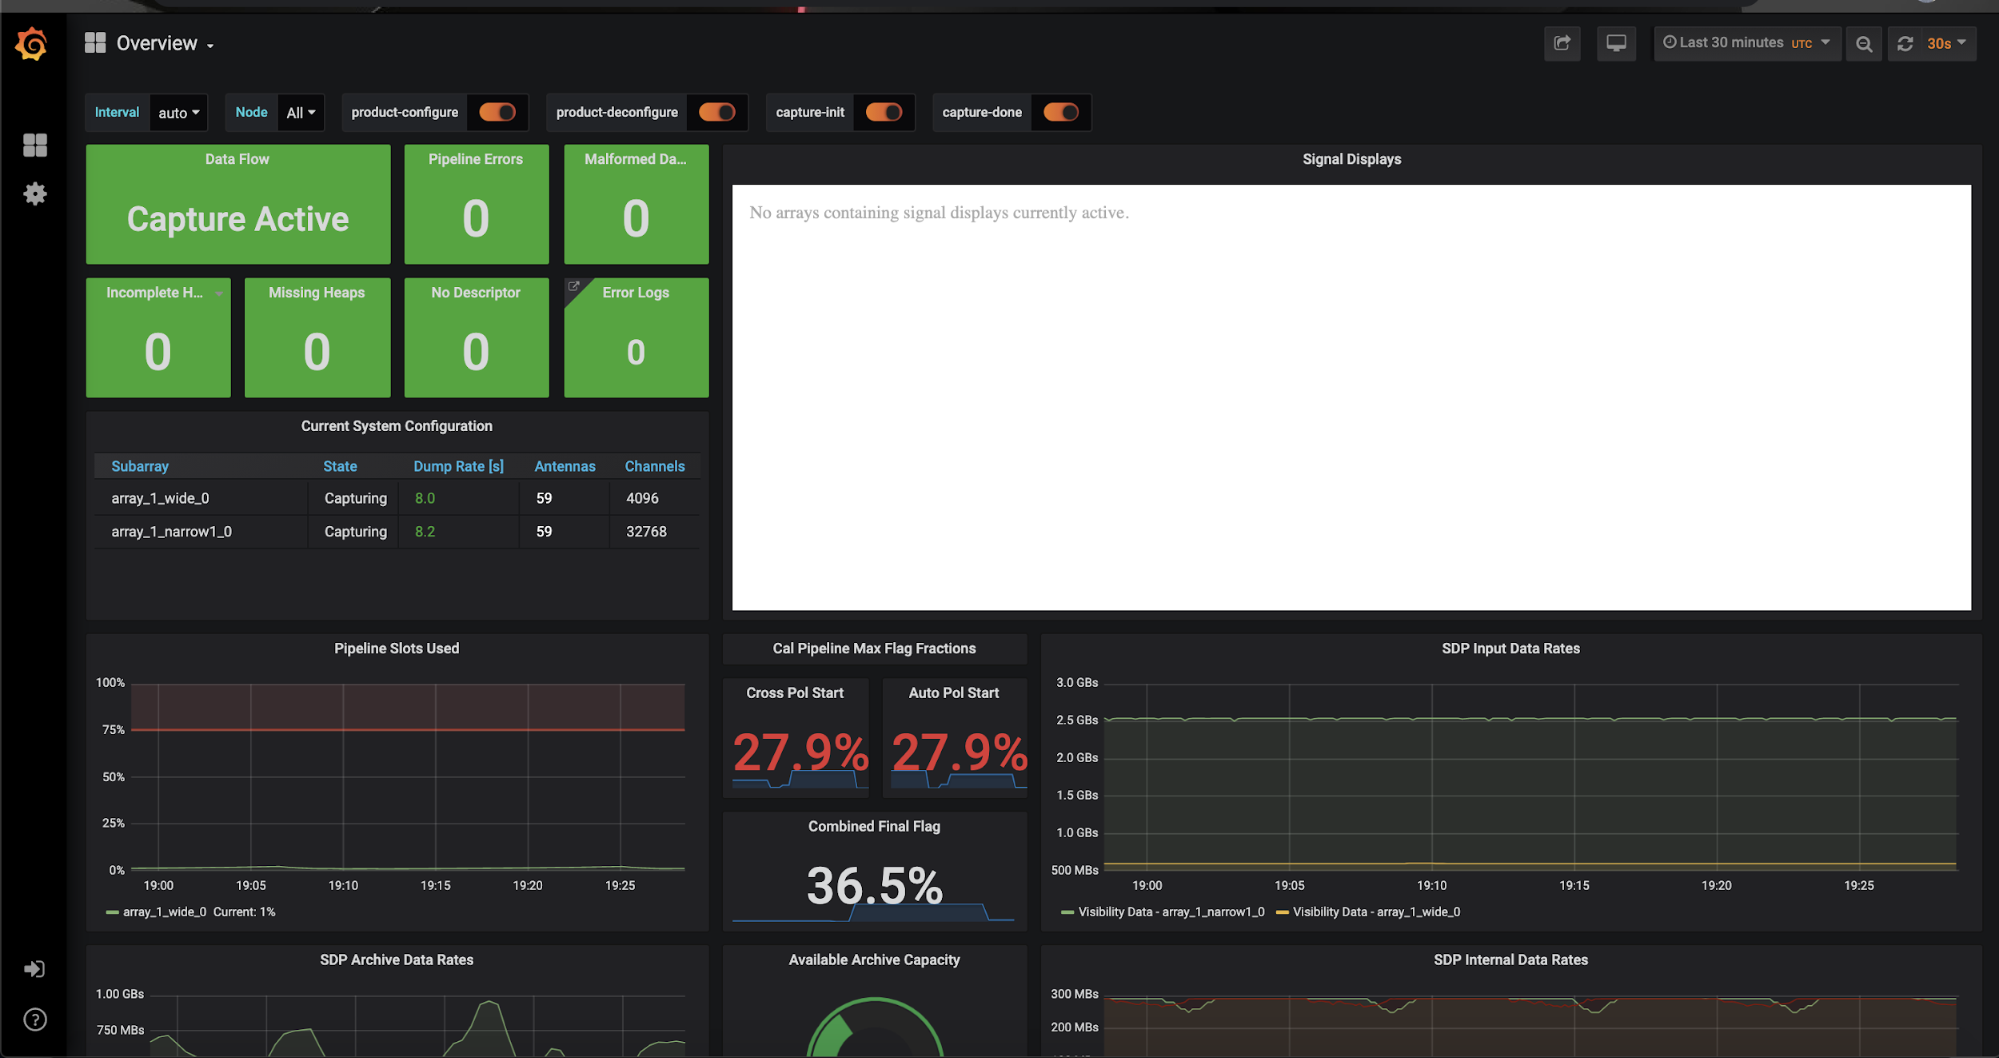
\includegraphics[scale=0.22]{Chapters/images/image15.png}
	
	%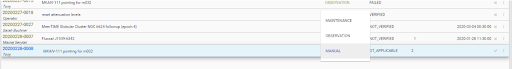
\includegraphics[resolution=100]{bur1.png}
	\caption{SDP Grafana dashboard without \sensor{no descriptors} errors}
	\label{fig:image15}
\end{figure}
\end{itemize}
If the no descriptor counts keep rising, the switch needs to be reloaded

\begin{itemize}
\item Tail the observation progress,see  \textbf{Figure}~\ref{fig:image100}.


\begin{figure}[H]
	\centering
	%\includegraphicsdpi{100}{{bur1.png}     
	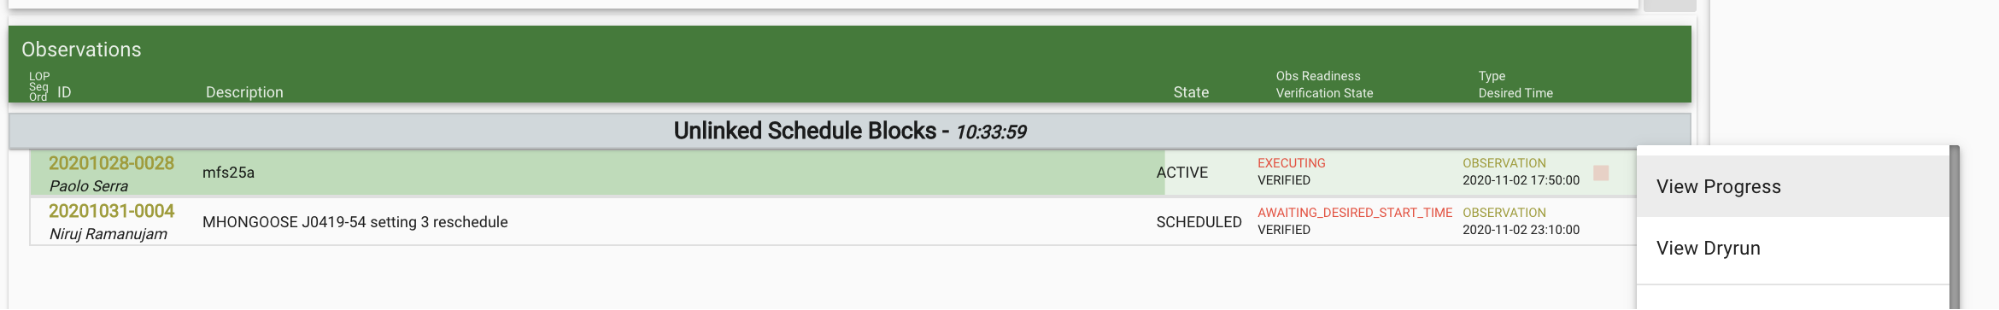
\includegraphics[scale=0.2]{Chapters/images/image100.png}
	
	%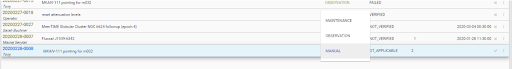
\includegraphics[resolution=100]{bur1.png}
	\caption{Observation progress log}
	\label{fig:image100}
\end{figure}


\item Load signal displays from  \url{ http://mc1.sdp.mkat.karoo.kat.ac.za:5004/}
You can also click on the link shown in \textbf{Figure}~\ref{fig:image126}, “Signal Display Dashboard ” under SDP resource.

\begin{figure}[H]
	\centering
	%\includegraphicsdpi{100}{}{bur1.png}     
	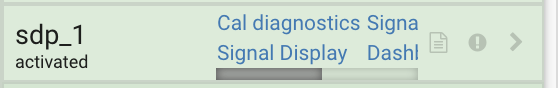
\includegraphics[scale=1]{Chapters/images/image126.png}
	
	%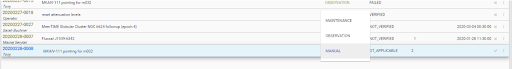
\includegraphics[resolution=100]{bur1.png}
	\caption{SDP signal display menu }
	\label{fig:image126}
\end{figure}

\item Type ‘load default2’ on the command line of the signal display \textbf{Figure}~\ref{fig:image50}.


\begin{figure}[H]
	\centering
	%\includegraphicsdpi{100}{}{bur1.png}     
	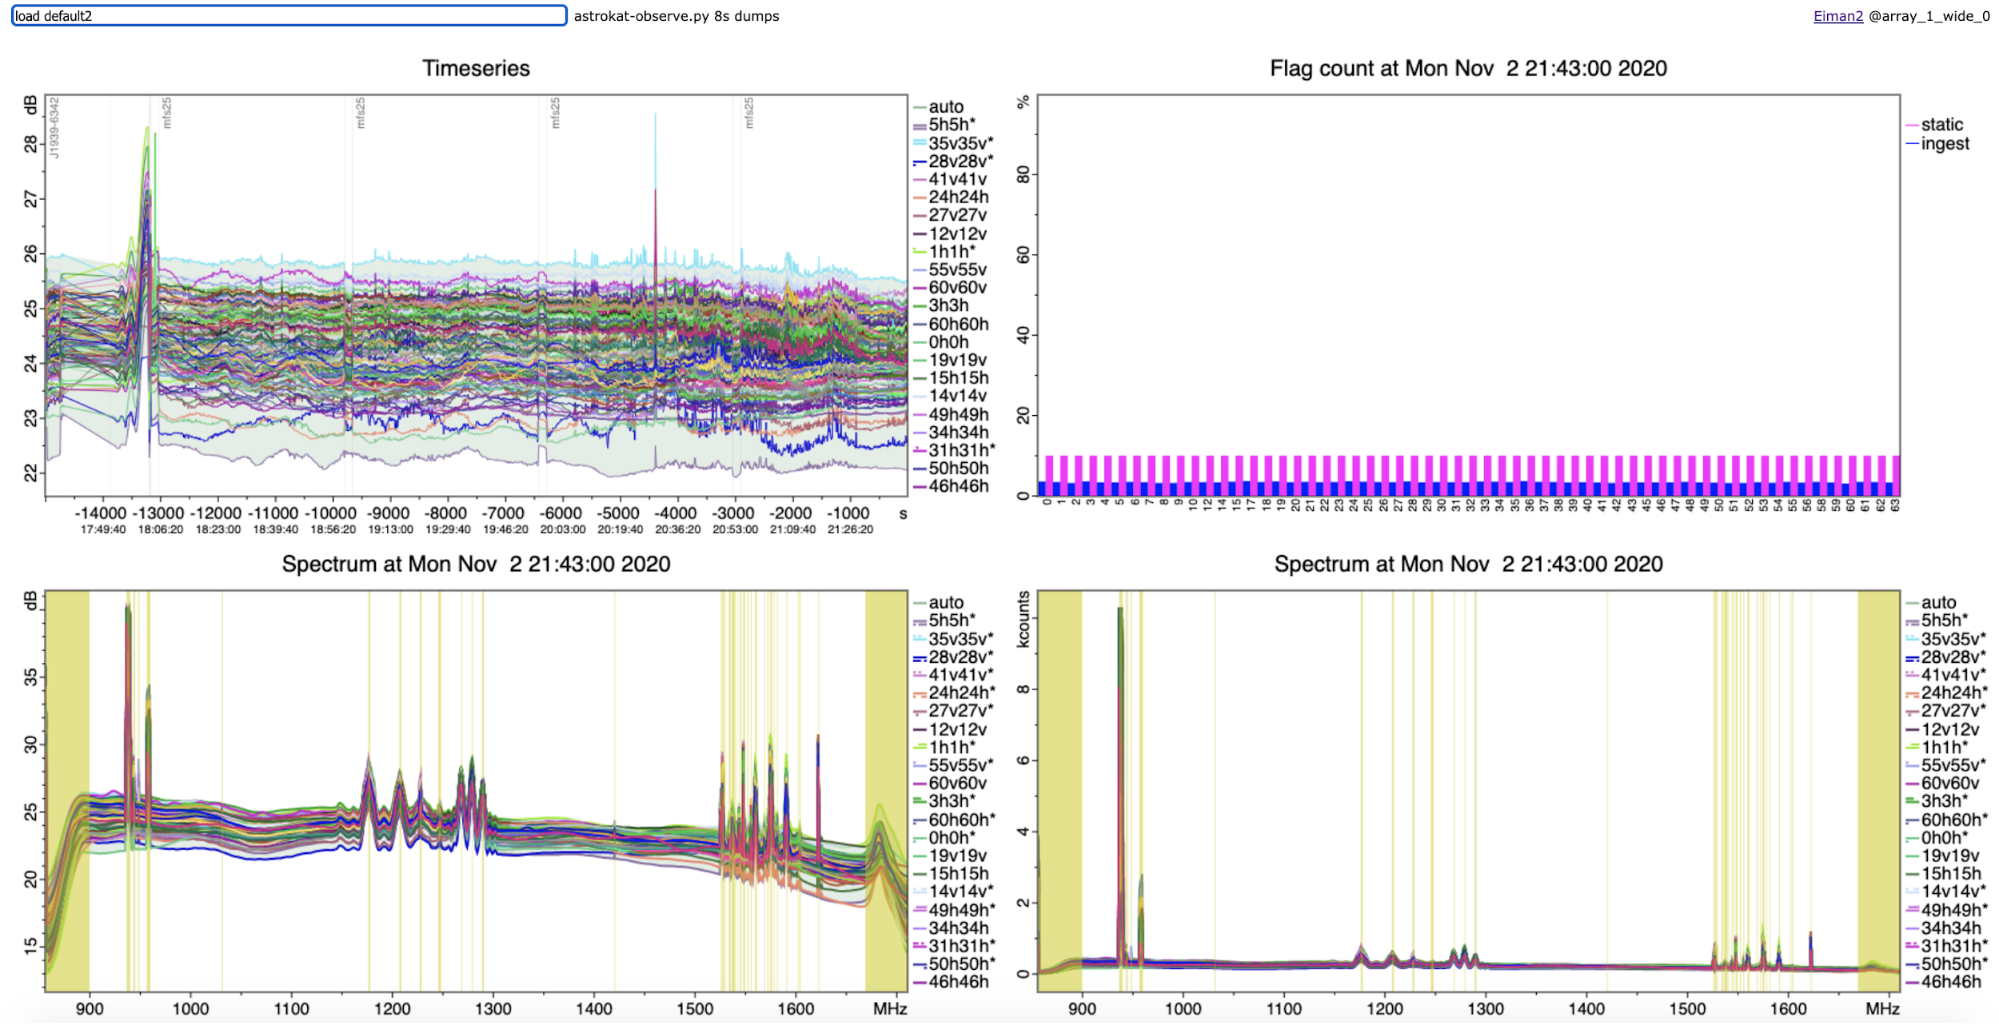
\includegraphics[scale=0.2]{Chapters/images/image50.png}
	
	%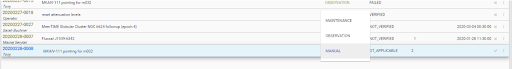
\includegraphics[resolution=100]{bur1.png}
	\caption{Default signal display}
	\label{fig:image50}
\end{figure}

If on the command line you type wtabhh  or wtabvv you will see displays similar to the one shown on Figure 53 and Figure 54 respectively. Here will be able to check for any faulty Receptors which are not phasing with other Receptors or may show noisy phase. 

\item{} Horizontal polarisations waterfall plot (wtabhh), this will display the waterfall in \textbf{Figure}~\ref{fig:image102}. polarisations. 
\clearpage

\begin{figure}[!thb]
	\centering
	%\includegraphicsdpi{100}{}{bur1.png}     
	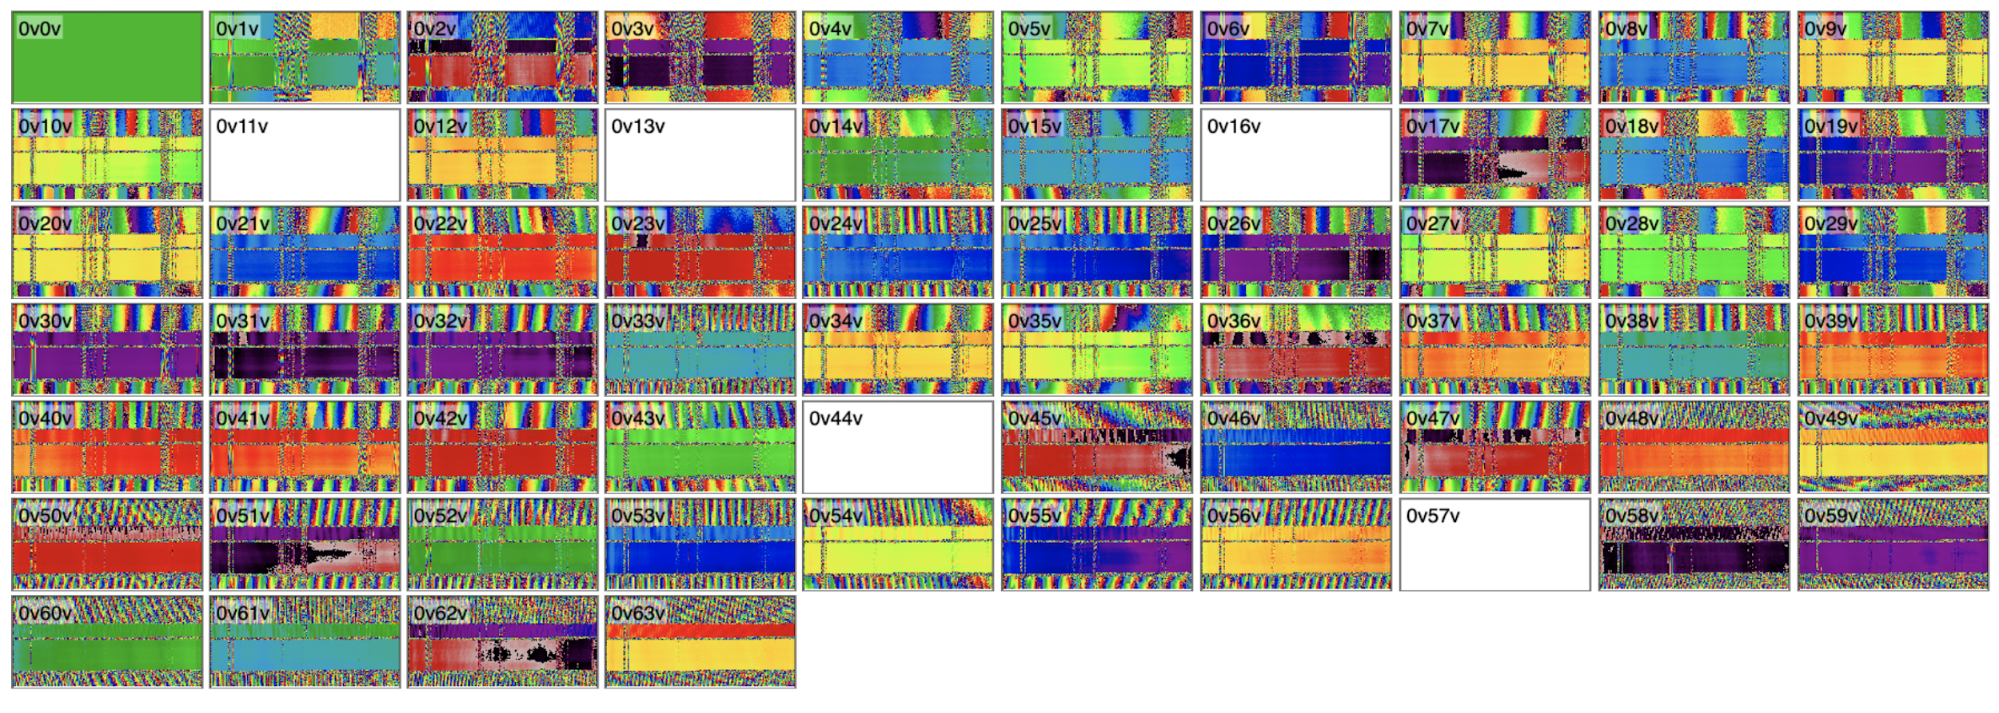
\includegraphics[scale=0.23]{Chapters/images/image102.png}
	
	%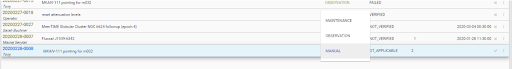
\includegraphics[resolution=100]{bur1.png}
	\caption{Horizontal polarisation plot (wtabhh)}
	\label{fig:image102}
\end{figure}

\item{} Vertical polarisation waterfall plot (wtabvv), see \textbf{Figure}~\ref{fig:image36}



\begin{figure}[!thb]
	\centering
	%\includegraphicsdpi{100}{}{bur1.png}     
	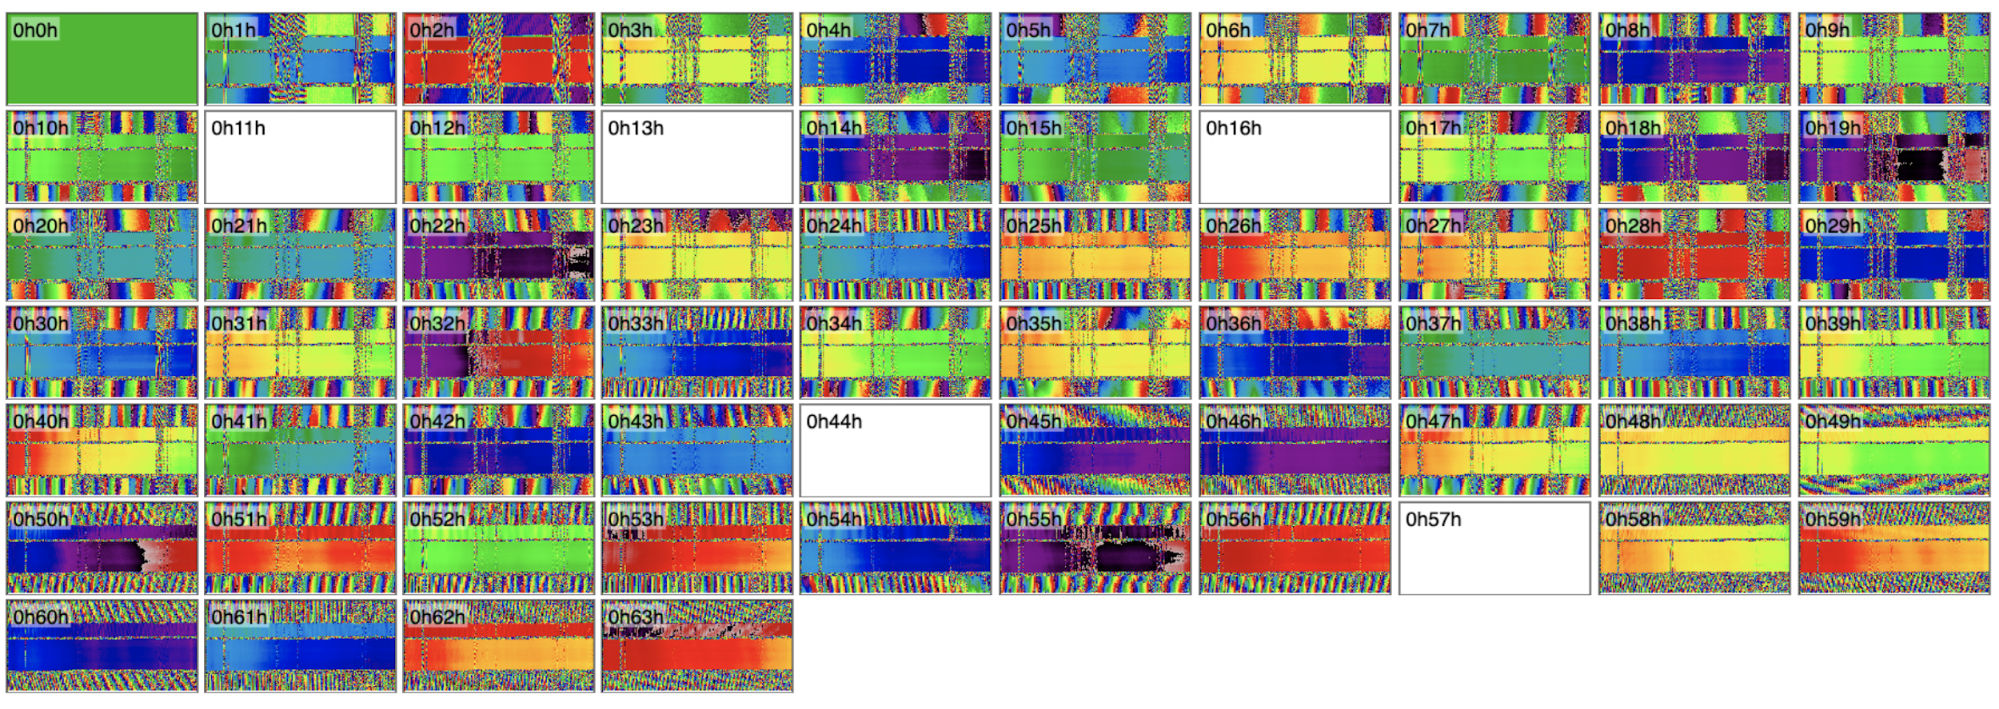
\includegraphics[scale=0.23]{Chapters/images/image36.png}
	
	%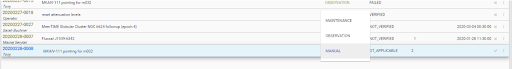
\includegraphics[resolution=100]{bur1.png}
	\caption{Vertical polarisation plot (wtabvv)}
	\label{fig:image36}
\end{figure}

If for any reason, there is an antenna that is not phasing with other antennas or the phase seems noisy, then it is better to check if that antenna is moving with other antennas. You can open the receptor pointing tab and check the status of that antenna as shown in \textbf{Figure}~\ref{fig:image76} 


\begin{figure}[H]
	\centering
	%\includegraphicsdpi{100}{}{bur1.png}     
	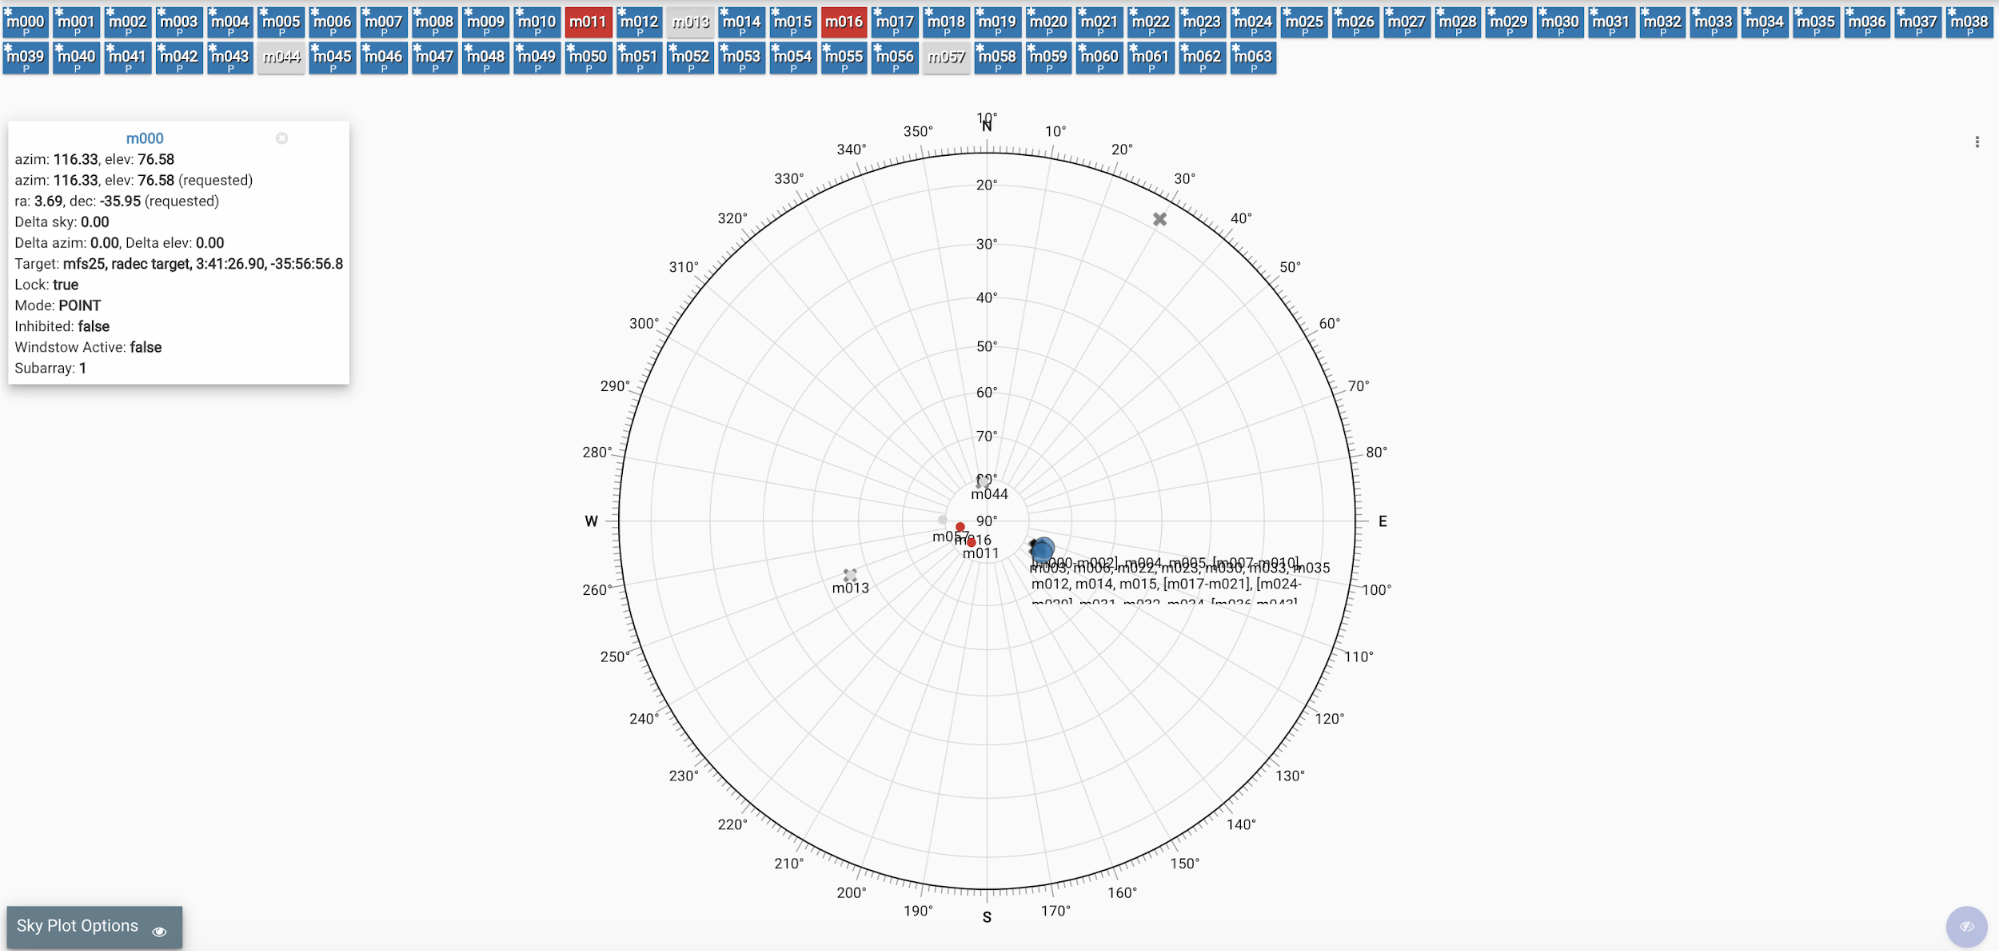
\includegraphics[scale=0.2]{Chapters/images/image76.png}
	
	%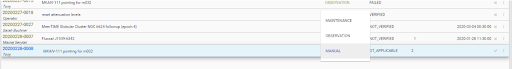
\includegraphics[resolution=100]{bur1.png}
	\caption{Receptor pointing plot}
	\label{fig:image76}
\end{figure}


This will indicate to you if the antenna is locked on to the target by showing ‘*’ on the antenna number, if it is not locked to the target there will be no ‘*’. It will be advisable to look at the sensor list of that antenna in questions. 
There may be other reasons for an antenna to have a noisy phase like a warm receiver, LNA switched off or CBF errors. 

After the array is built  you can select “Sensor Groups” from the CAM GUI landing page and select critical observation sensors. This will list all the critical sensors that are required to be safe and okay for the observation as shown in \textbf{Figure}~\ref{fig:image125}.  

\end{itemize}

\begin{figure}[H]
	\centering
	%\includegraphicsdpi{100}{}{bur1.png}     
	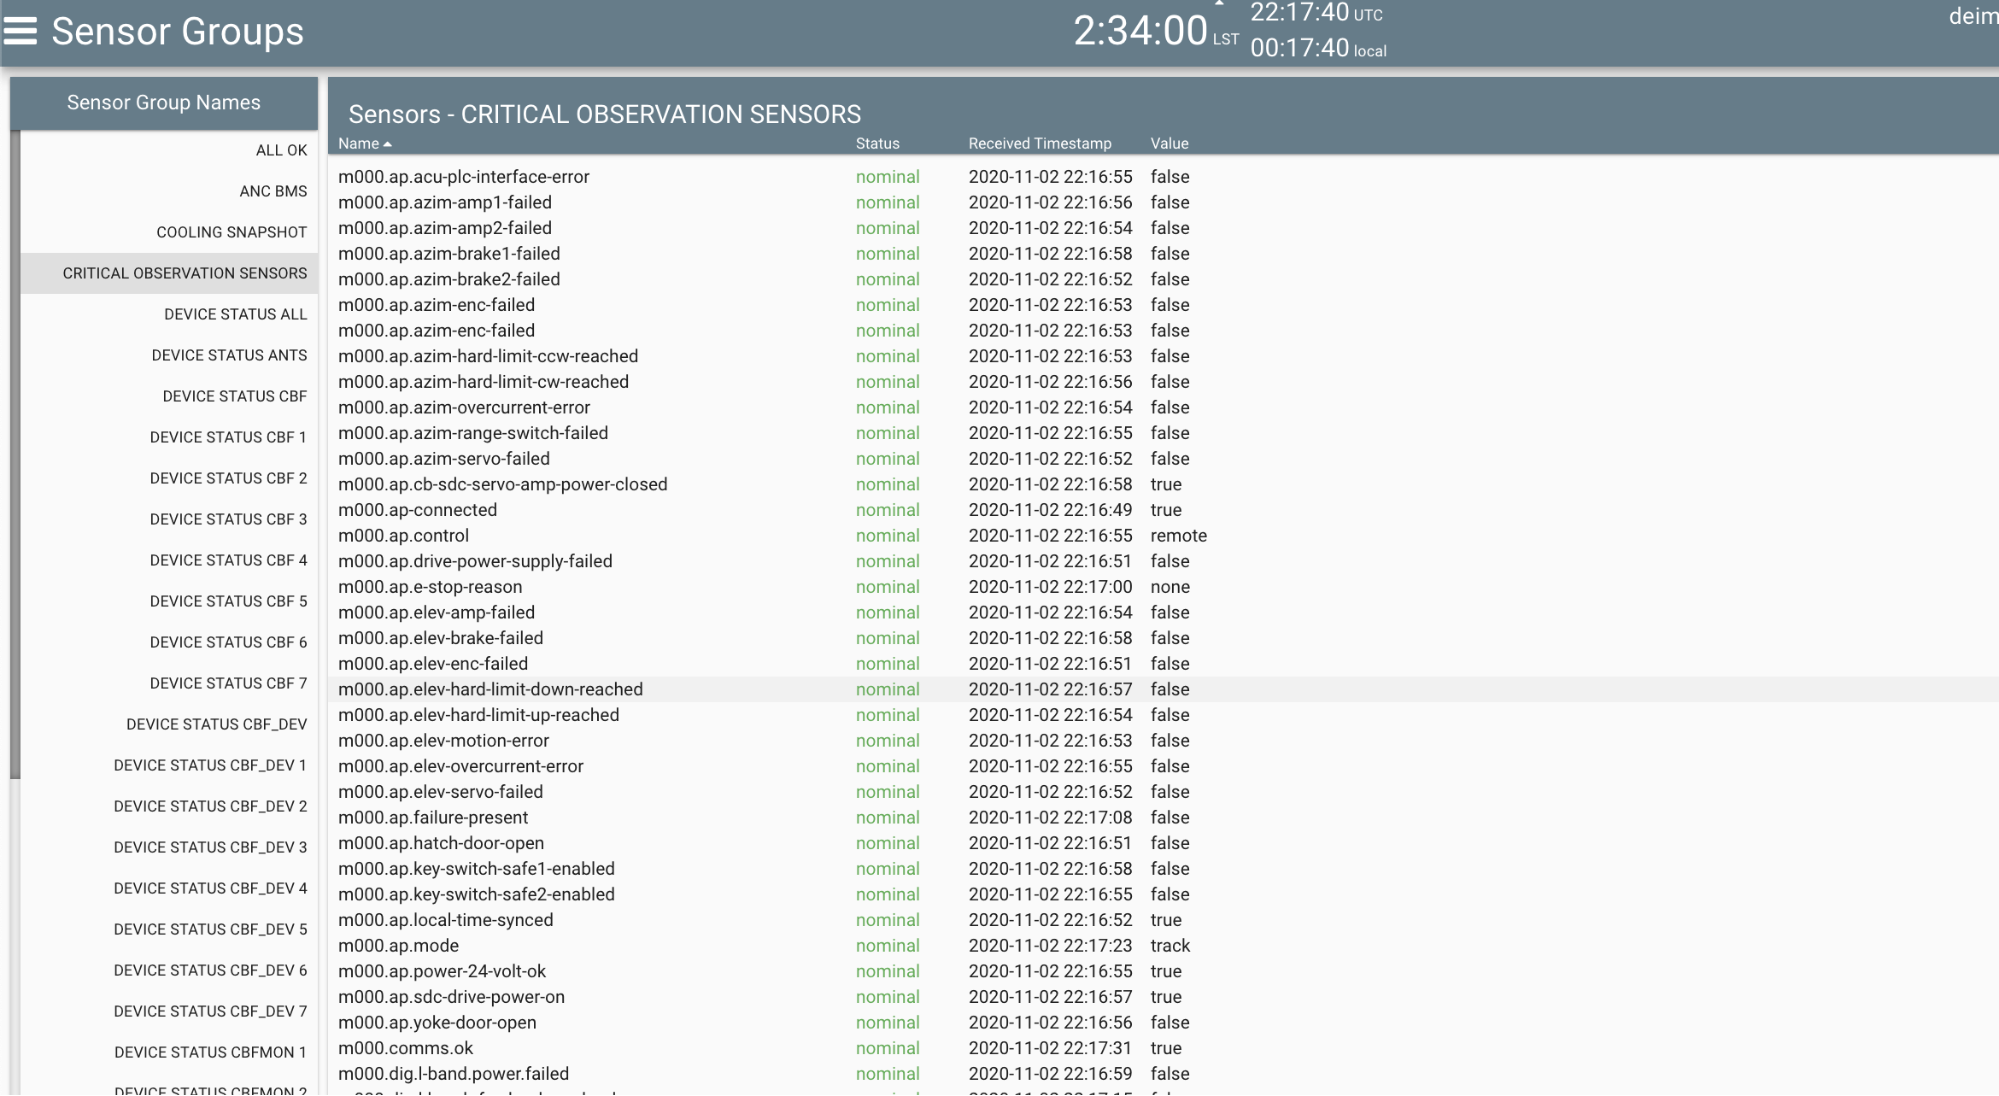
\includegraphics[scale=0.2]{Chapters/images/image125.png}
	
	%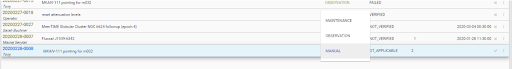
\includegraphics[resolution=100]{bur1.png}
	\caption{CAM GUI List of critical sensors}
	\label{fig:image125}
\end{figure}


\section{ Monitoring SDP}

In order to see the status of the SDP subsystem after the array is built and the observation is running you can  start up the Science Processor dashboard (see \textbf{Figure}~\ref{fig:image123}). This dashboard called Grafana will give you all the information about the health of the SDP system and also data flow from CBF to SDP. 



\begin{figure}[H]
	\centering
	%\includegraphicsdpi{100}{}{bur1.png}     
	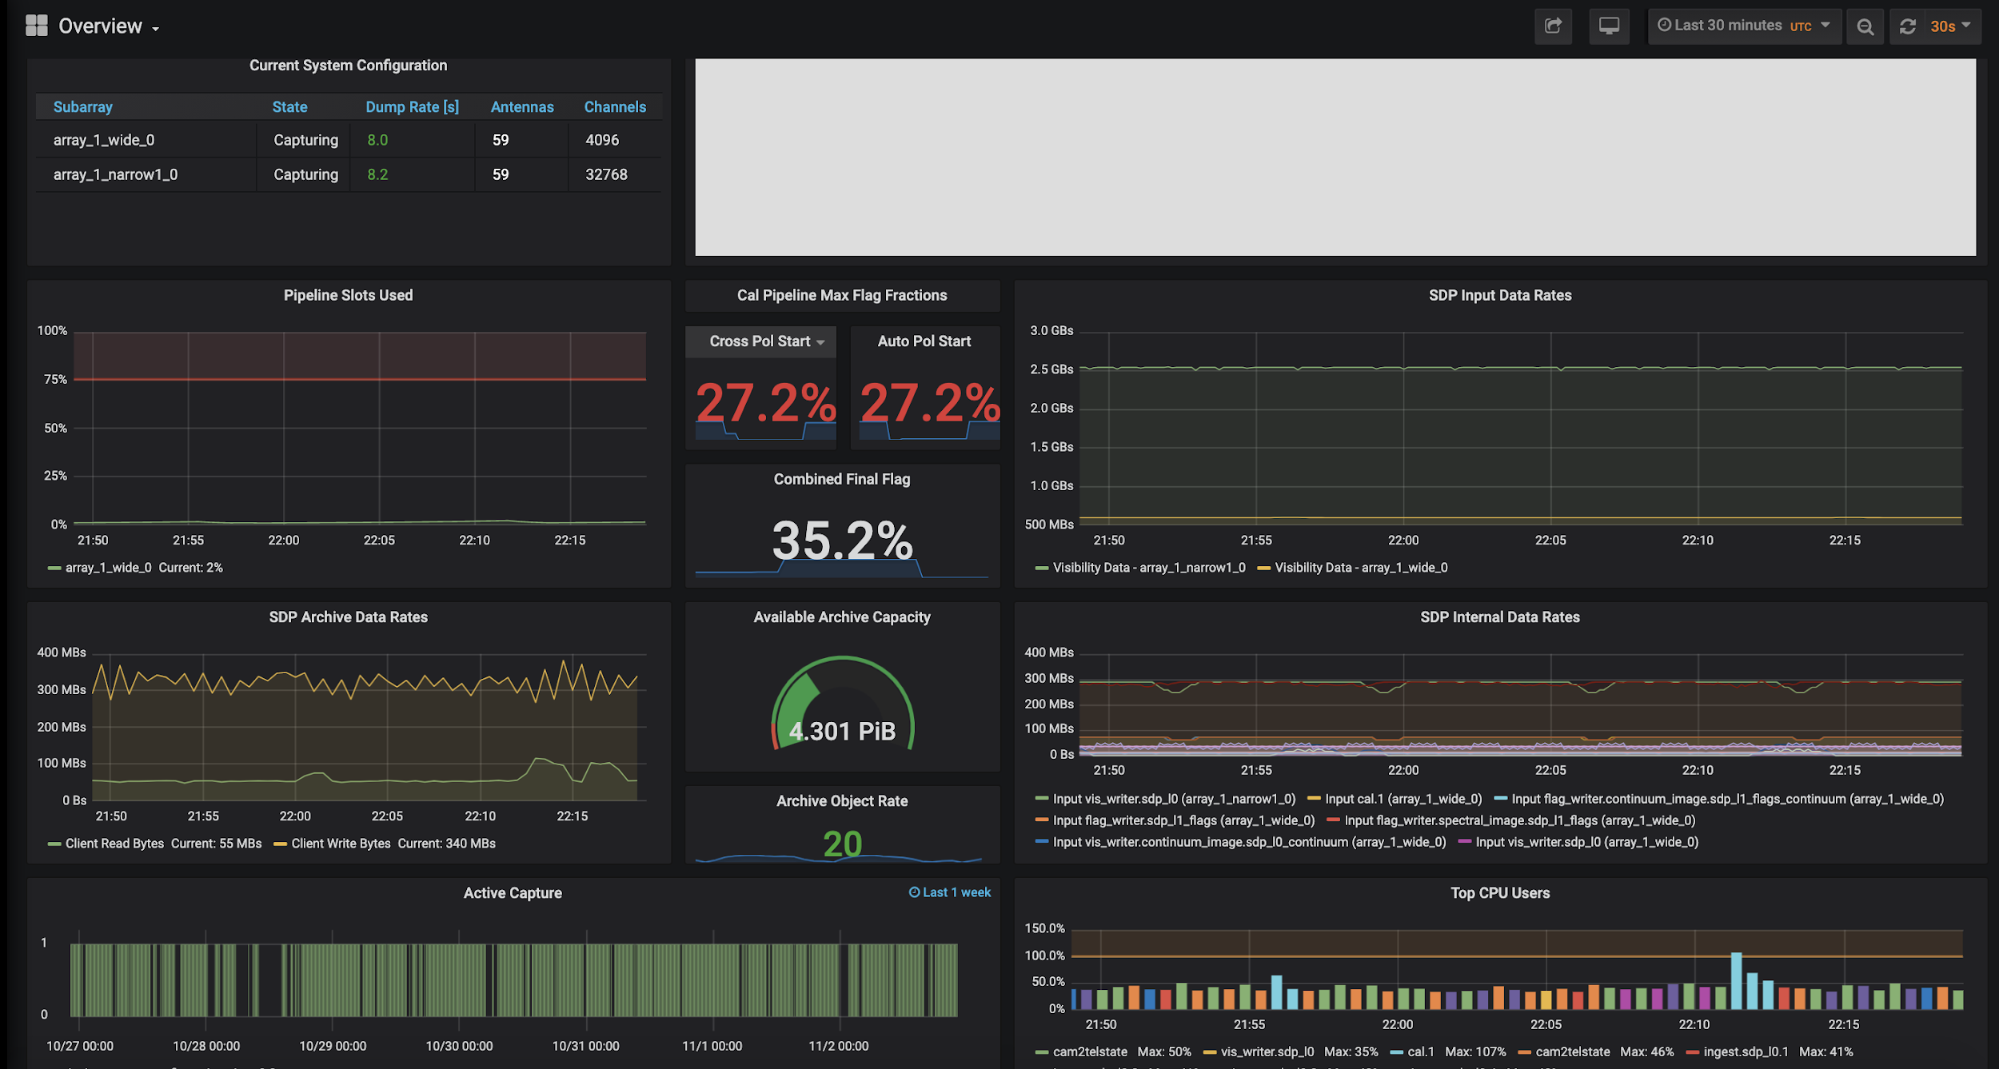
\includegraphics[scale=0.23]{Chapters/images/image123.png}
	
	%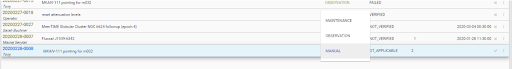
\includegraphics[resolution=100]{bur1.png}
	\caption{Grafana dashboard for SDP status}
	\label{fig:image123}
\end{figure}


There are more documents that have been written which describe procedures to be followed by operators when SDP encounters errors. 

\section{Monitoring Receptors}

Any faults on APs can be monitored by running the ipython session on obs.mkat.ka
\begin{lstlisting}[style=DOS]
ssh kat@obs.mkat.karoo.kat.ac.za

ipython

import katuilib
configure()

ant_inactive = sorted([ant.name for ant in kat.ants if ant.name \
in kat.katpool.sensor.resources_in_maintenance.get_value()])
ant_list = ''


for a in ant_inactive: ant_list = ant_list + a[2:] + '|'

ant_list = ant_list[:-1]

ap_sensors="(^m0(?!(%s|2(1|7).ap.ridx.hard.limit.*reached$)).*(connected|local.time|fail*|limit|(cb.*(sdc|pdc|digitiser1|receiver1|pump))|error|hatch|yoke|switch|ap.*mode|drive.power|read.error.count|rxl.(rfe1.temperature|lna.*.power.enabled)|(he.compressor.device)|windstow.active))|(dmc.*epoch)" % ant_list

kat.print_sensors(ap_sensors, strategy='period', status='warn|error|failure|unreachable')
\end{lstlisting}




This should generate the output as shown in \textbf{Figure}~\ref{fig:image124}.



\begin{figure}[H]
	\centering
	%\includegraphicsdpi{100}{}{bur1.png}     
	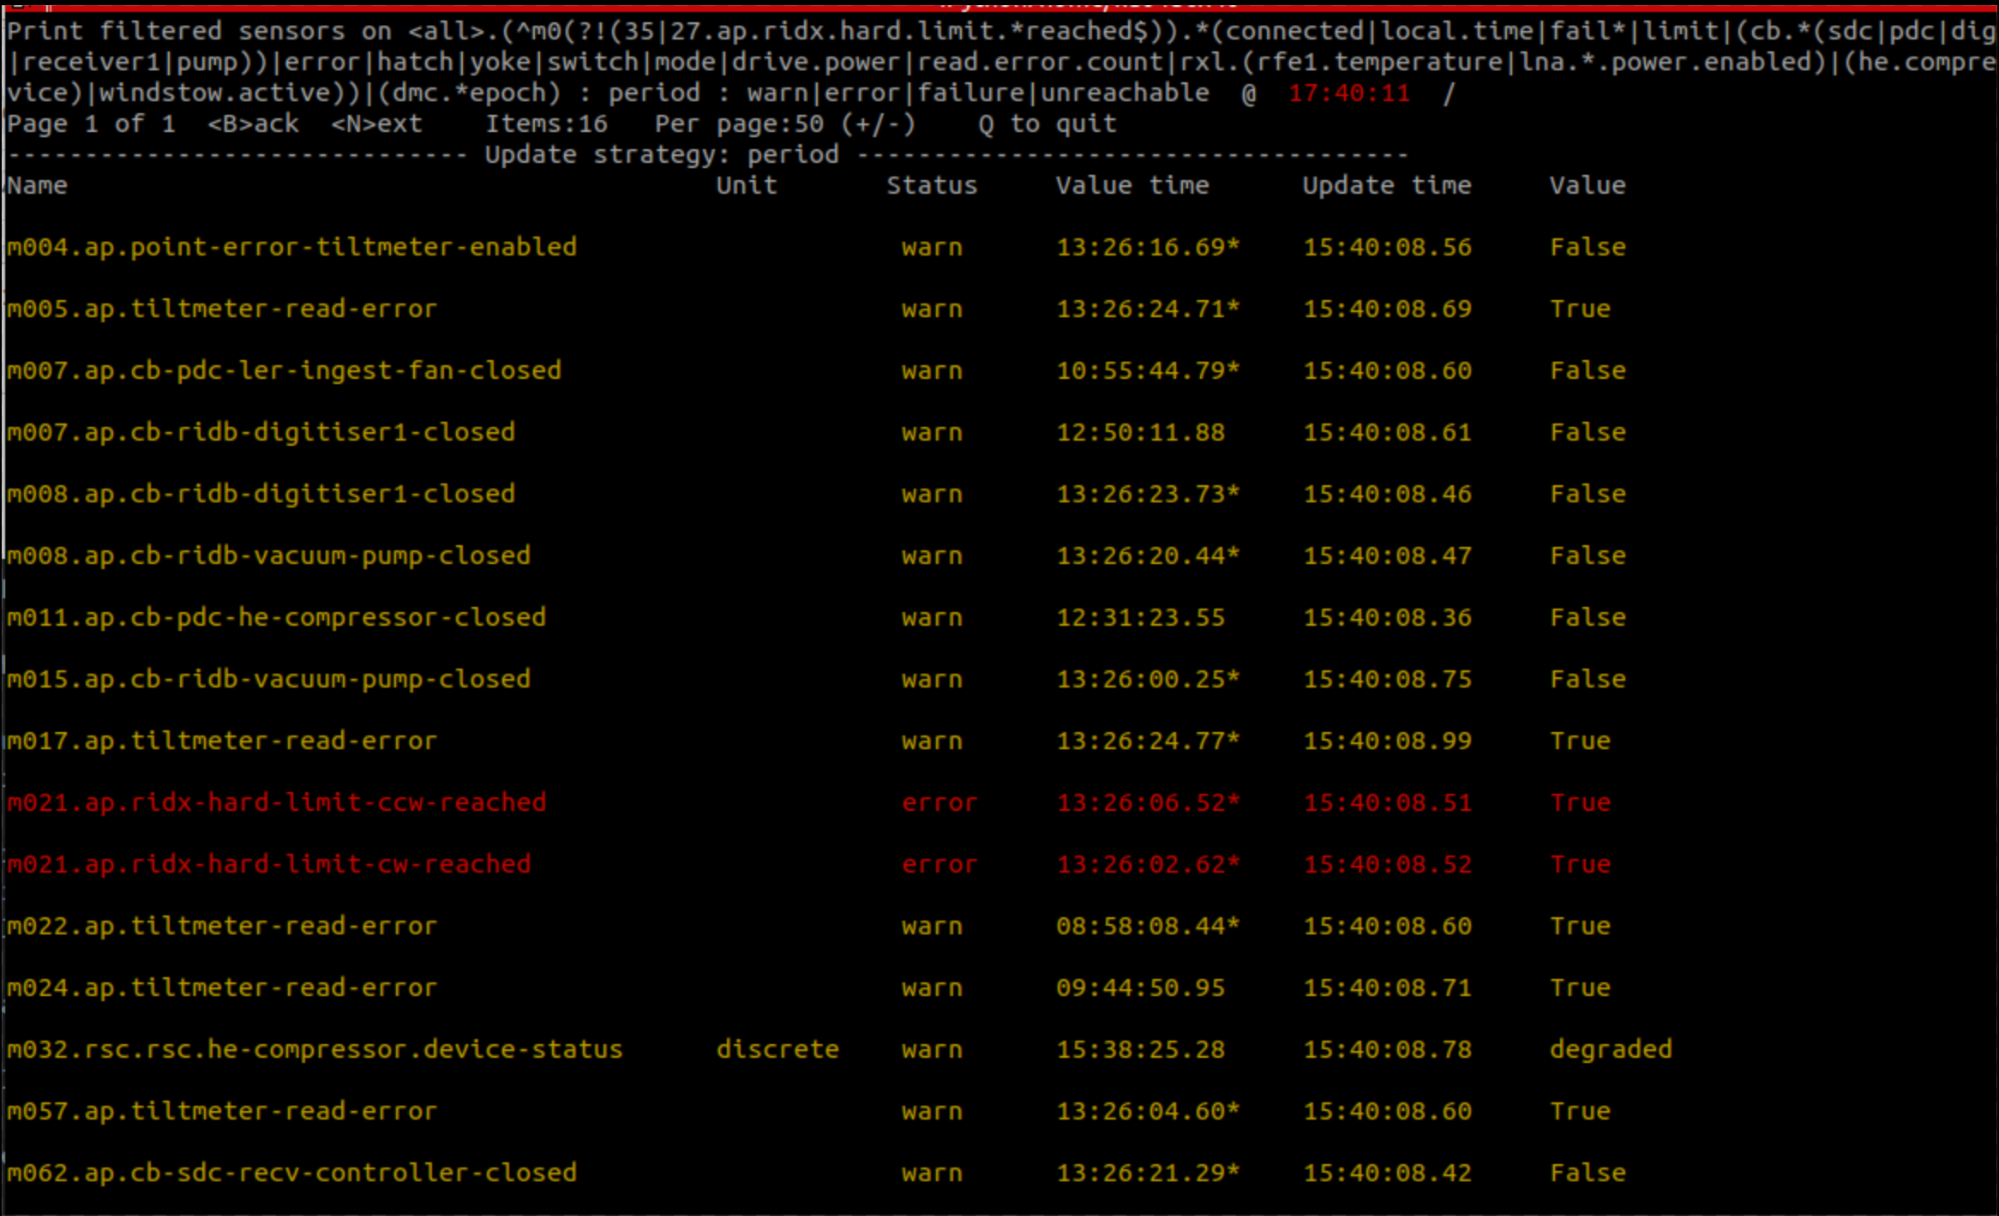
\includegraphics[scale=0.23]{Chapters/images/image124.png}
	
	%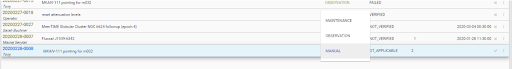
\includegraphics[resolution=100]{bur1.png}
	\caption{Output of antenna monitoring script}
	\label{fig:image124}
\end{figure}


\textbf{AP fault finding during observation:}
\begin{itemize}

\item  \textcolor{blue}{Exclude APs in Maintenance on Critical Observation Sensors}

Critical Observation Sensors is comprised of observation critical sensors. Sometimes receptors in maintenance flood the page when sensors transition to several non-nominal states, e.g. error, warn, failure, and unreachable. As this behavior is expected with maintenance, better to filter these receptors using regular expressions.  The example of how to do this is shown below in \textbf{Figure}~\ref{fig:image120}.

\item \textcolor{blue}{Filter out nominal sensors (default setting)}

Notice m024 sensors are mainly occupying the page as it is worked on. This could potentially mask a set of active APs in the process. Moreover, m017 and m018 digitizers are inactive, would you like to constantly monitor that? Of course not.



\begin{figure}[!thb]
	\centering
	%\includegraphicsdpi{100}{}{bur1.png}    1206.png}
	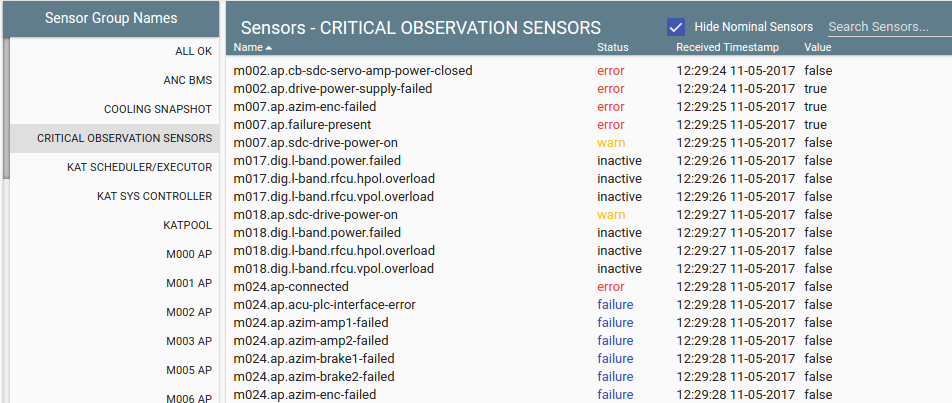
\includegraphics[scale=0.33]{Chapters/images/image120.png}
	%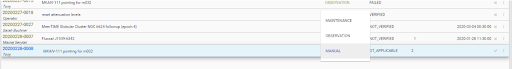
\includegraphics[resolution=100]{bur1.png}
	\caption{Critical observation sensors with hidden nominal sensors}
	\label{fig:image120}
\end{figure}

\item \textcolor{blue}{Excluding receptors}

For instance,\component{ m017, m018, m024, m025} and \component{m063} will be excluded. The expression is: m0(?!(17|18|24|25|63)) as shown in \textbf{Figure}~\ref{fig:image88}

\end{itemize}

\begin{figure}[!thb]
	\centering
	%\includegraphicsdpi{100}{}{bur1.png}     
	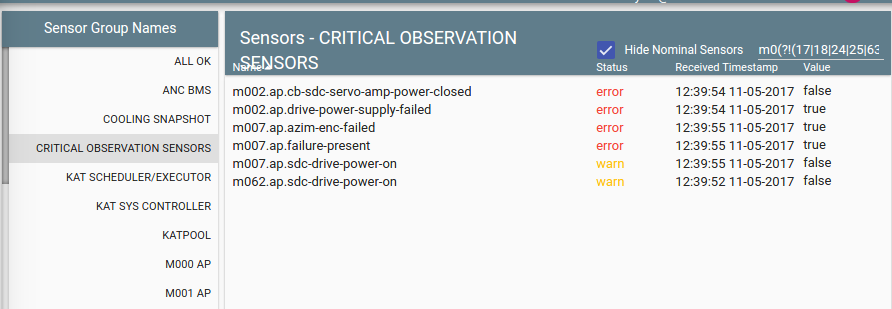
\includegraphics[scale=0.34]{Chapters/images/image88.png}
	
	%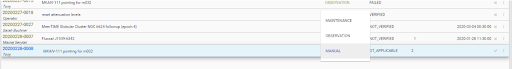
\includegraphics[resolution=100]{bur1.png}
	\caption{Critical sensor list filtered by AP names}
	\label{fig:image88}
\end{figure}


\section{ Monitoring CBF}
In order to monitor the status of the Correlator Beamformer (CBF) system, load the cbf mon\_1 plot on the GUI to monitor CBF health as shown in \textbf{Figure}~\ref{fig:image122}. 


\begin{figure}[H]
	\centering
	%\includegraphicsdpi{100}{}{bur1.png}     
	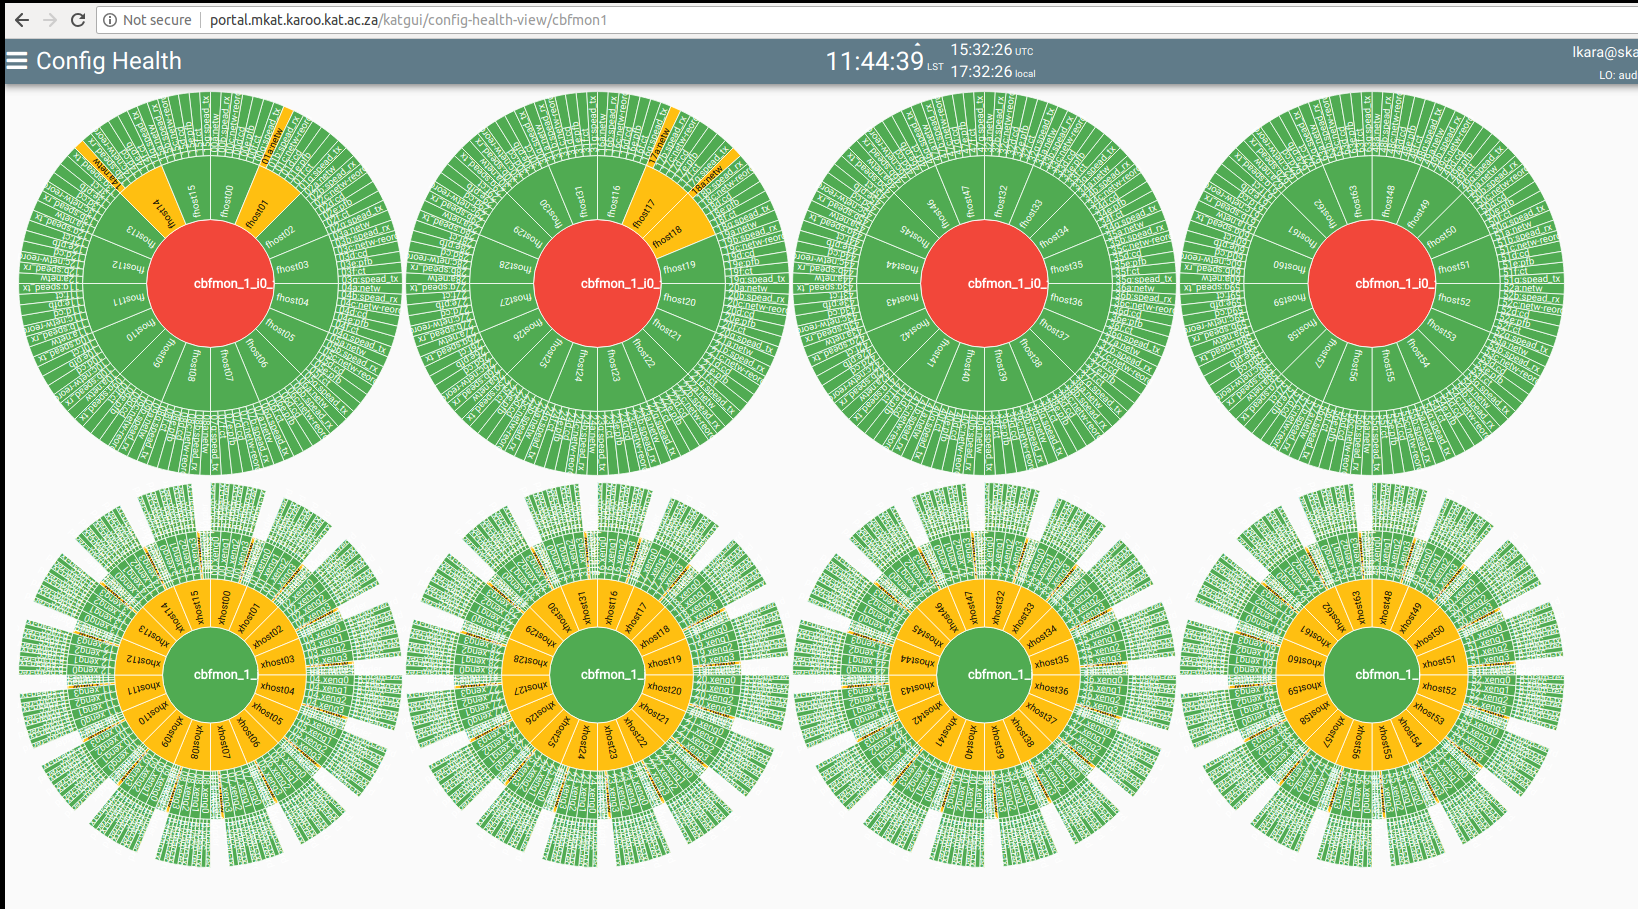
\includegraphics[scale=0.23]{Chapters/images/image122.png}
	
	%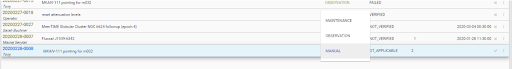
\includegraphics[resolution=100]{bur1.png}
	\caption{CBF monitor pie plots}
	\label{fig:image122}
\end{figure}

This will drill down to all the sensors of the CBF and will show warnings and alarms of each Skarab board. The dashboard will give you all the f-hots and x-hosts used in the array. Note that this display only becomes live after the subarray is built. 
It is important to know that for a normal wide band observation with 64 antennas, there will be 128 Skarabs used. 64 are used for F-engines and another 64 are used for X-engines.  But for wide band and narrow band, a total of 200 skarabs will be used for this observation. 

The alternative to looking at the CBF health status as shown in \textbf{Figure}~\ref{fig:image122} by using the following link:
\url{http://cbf-nuc2.cpt.kat.ac.za/cmc1/array\_1.wide}

If you want to see more CBF logs  you can monitor them by running cmc-top on the obs machine.
\begin{lstlisting}[style=DOS]
cmc-top cmc1.cbf.mkat.karoo.kat.ac.za:7147


\end{lstlisting}

\section{ Monitoring Digitiser }
\subsection{ Digitiser Spectrometer Overflows}

This is not a critical fail - it just reports that the power into the spectrometer causes the FFT to overflow (but it still works - much like an ADC saturation) - this is not supposed to happen, but it might be that the fft\_shift was decreased, causing this. 

This issue is that fft\_shift is set to 0 on a few digitisers (as opposed to 0xfffffffff) - this will cause FFT overflows. Must be at least 7. This is TBD at this stage.

\subsection{ Digitiser Deng Overflows}
When building a subarray, network problems (like the network interface crashing) can cause the digitiser to capture-start incorrectly, resulting in a deng overflow error. The f-host connected to this digitiser also a lot of times will give network reorder errors and thus appear red in the cbfmon1 plot. When you free the subarray, the error clears, but will appear again if you build a subarray again with the affected digitiser.

When this error occurs, the digitiser needs to be reconfigured:
Mark the digitiser absent.
Contact the digitiser team to reconfigure the problematic digitiser.
Mark the digitiser ready again.

\subsection{ Digitiser Power Failed}
This sensor tracks only if the system has been rebooted/lost power unexpectedly. This could mean that the digitiser has been power cycled somehow.

Since the sensor tracks lost power, it will not clear even if the digitiser has been powered again and works nominally. To clear the error:
Mark the digitiser absent.
Mark the digitiser ready again. 
\section{ Monitoring Receiver }
\subsection{ Drain current errors on the receiver}
If the drain current power drops by a few mA on either the h-pol or the v-pol or both, then it will go into error. When that happens:
Power cycle the LNA of that AP.
Normally this will solve the problem, otherwise contact Ben Jordaan
\section{ Monitoring of Weather and Wind Sensors}
\subsection{ Weather Information}
There are three weather stations consisting of wind speed, wind direction, temperature and barometric pressure instruments that are installed next to the antennas. Operators are required to monitor the wind conditions as high wind conditions may cause damage to the AP.  The weather information is also used for observations so it is important that operators ensure that weather instruments are working at all times. Inorder to monitor weather, click on Weather tab under sensors on the CAM GUI as shown in \textbf{Figure}~\ref{fig:image67}



\begin{figure}[!thb]
	\centering
	%\includegraphicsdpi{100}{}{bur1.png}     
	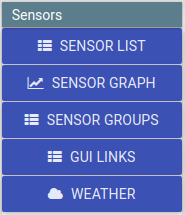
\includegraphics[scale=0.73]{Chapters/images/image67.png}
	
	%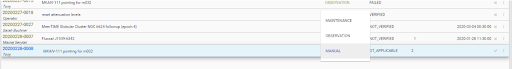
\includegraphics[resolution=100]{bur1.png}
	\caption{CAM GUI weather button }
	\label{fig:image67}
\end{figure}

You will be able to view weather for the past 2 hours and up to a week interval. In the graph in \textbf{Figure}~\ref{fig:image56} there is a dotted line which shows the minimum and maximum wind speed threshold. If the wind speed is above minimum threshold for sustained period, the antenna will go to a stow position >90 deg in elevation to protect themselves from damage due to high winds.  If the wind gust goes above upper limit the antennas will store immediately.



\begin{figure}[!thb]
	\centering
	%\includegraphicsdpi{100}{}{bur1.png}     
	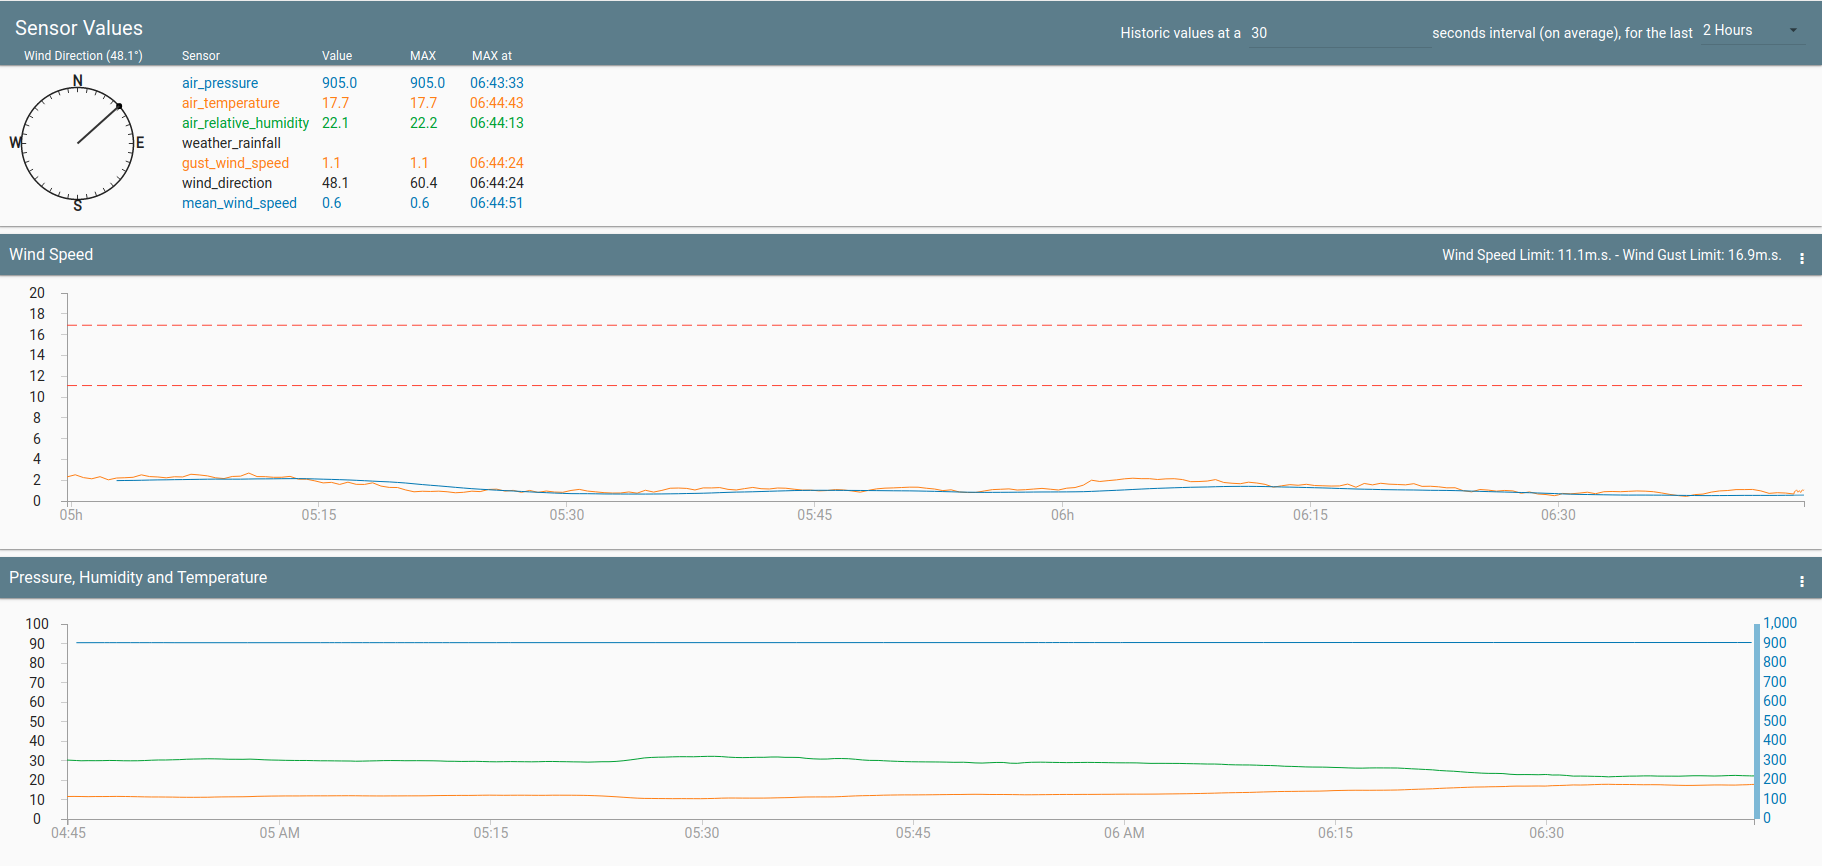
\includegraphics[scale=0.23]{Chapters/images/image56.png}
	
	%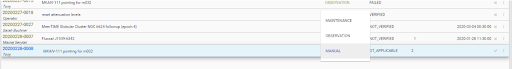
\includegraphics[resolution=100]{bur1.png}
	\caption{CAM GUI Weather plots}
	\label{fig:image56}
\end{figure}

\subsection{ Weather Station Errors}
ANC\_Wind\_Reporting\_Failure
The alarm is normally raised because the monitor process(mon\_proxy00) is unable to sync with the ANC proxy and get the latest values. Because we do not know the latest value of the wind speed we raise an alarm: ANC\_Wind\_Reporting\_Failure
Solution to try to solve the issue: Restart the ANC proxy and the mon\_proxy00 process. Should the Restart not work, call CAM Support.

ANC\_Wind\_Gust
The alarm is normally raised because CAM was able to read from the device that the wind speed sensor exceeds the max speed set.
Solution: Nothing, except to wait for the wind speed to subside.




\section{ Monitoring BMS Sensors in KAPB}
\subsection{ BMS} 
The BMS sensors are made to assist operators in monitoring the KAPB building that houses all the racks  such as SP, APSUSE, TUSE, CBF, PTUSE, FBFUSE among others. The KAPB needs to be kept at an optimum temperature and RFI free at all times. 
Currently the Building Management System  link to CAM is still under maintenance. \\
To check the BMS sensors:\\
In the GUI, click on the sensor list tab>under components, click \sensor{ANC} $>$ search "bms" or 
\url{http://portal.mkat.karoo.kat.ac.za/katgui/sensor-list?component=anc}
\subsection{ KAPB PDU Temperatures}
Due to HVAC work done in the Karoo Array Processor Building (KAPB), the interface between the HVAC units and the Building Management System (BMS) is currently broken so the BMS guys are not able to monitor the temperature in the KAPB.  So when you are LO please check periodically temperature sensors connected to the following Power Distribution Units (PDU). They are using this just to make sure that the correct temperature is maintained and if violated might cause temperature drifts on the Masers.

If the alarms come through please send email to Andre and Dave they will know what to do.

In order to access these KAPB PDU Temperatures you need to login to observium.
The username is guest and password is guest or click the links below.
A6 PDU(Hot floor level) has an alarm but warning = 24 deg and alarm = 26 deg http://observium.kat.ac.za/graphs/to=1595401736/device=153/type=device\_temperature/from=1595315336/legend=yes/
C11 PDU(Cold below floor) has an alarm but warning = 20 deg and alarm = 22 deg
http://observium.kat.ac.za/graphs/to=1595402069/device=179/type=device\_temperature/from=1595315669/legend=yes/
D12 PDU has no alarm, warning = 21 deg and alarm 23 deg (this is what we must prevent, report before the temp rises to 23 deg. 
http://observium.kat.ac.za/graphs/to=1595399299/device=479/type=device\_temperature/from=1594794499/legend=yes/

\section{ Inspecting Telescope Network Nodes}
\subsection{ Pinging Nodes With a Script}
The script must be run on the ops server. It takes one of the three command-line options to the network on a subsystem-selection basis.

Start by logging onto the ops server and see the output in \textbf{Figure}~\ref{fig:image127}
\begin{lstlisting}[style=DOS]
ssh kat@ops.kat.ac.za
cd ops\_team\_sw/utilities/mKat/
Usage helper: run 
./check\_mkat\_net.sh

\end{lstlisting}


\begin{figure}[!thb]
	\centering
	%\includegraphicsdpi{100}{}{bur1.png}     
	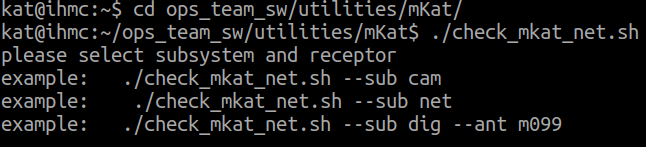
\includegraphics[scale=0.63]{Chapters/images/image127.png}
	
	%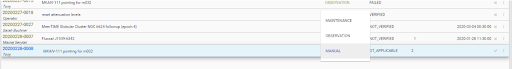
\includegraphics[resolution=100]{bur1.png}
	\caption{Output of \_net.sh script $-$ Spine switch status}
	\label{fig:image127}
\end{figure}


To test all CAM nodes, run the following command and see output in \textbf{Figure}~\ref{fig:image55}
\begin{lstlisting}[style=DOS]
./check\_mkat\_net.sh --sub cam

\end{lstlisting}




\begin{figure}[!thb]
	\centering
	%\includegraphicsdpi{100}{}{bur1.png}     
	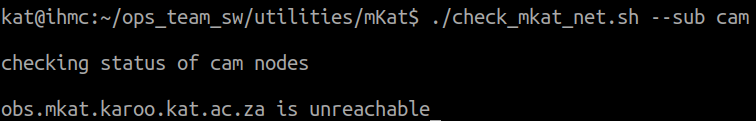
\includegraphics[scale=0.55]{Chapters/images/image55.png}
	
	%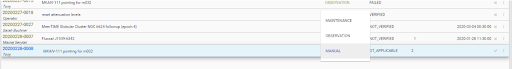
\includegraphics[resolution=100]{bur1.png}
	\caption{Output of \_net.sh script $-$ All CAM nodes status}
	\label{fig:image55}
\end{figure}


To test ping the link to site and all subsystem spine switches, run the folloing command and see output in \textbf{Figure}~\ref{fig:image117}:
\begin{lstlisting}[style=DOS]
./check\_mkat\_net.sh --sub net

\end{lstlisting}



\begin{figure}[H]
	\centering
	%\includegraphicsdpi{100}{}{bur1.png}     
	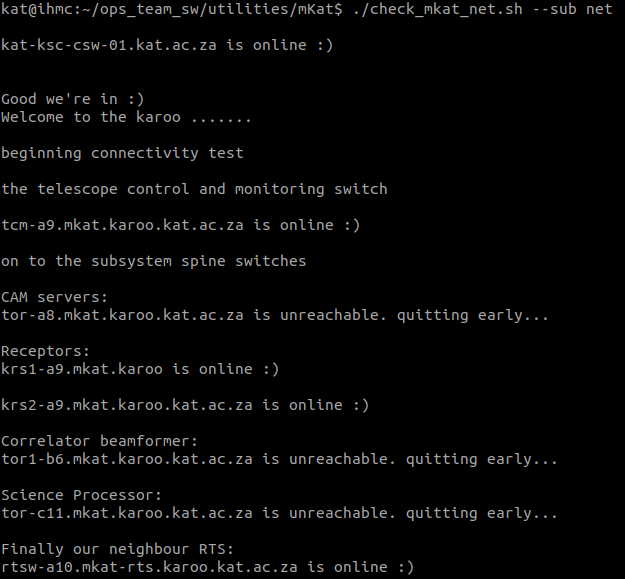
\includegraphics[scale=0.53]{Chapters/images/image117.png}
	
	%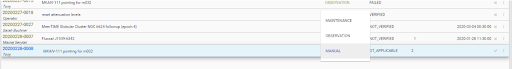
\includegraphics[resolution=100]{bur1.png}
	\caption{Output of \_net.sh script $-$ Spine switch status}
	\label{fig:image117}
\end{figure}


To check if a digitiser is online, run the folowing command and see the output in \textbf{Figure}~\ref{fig:image75}:
\begin{lstlisting}[style=DOS]
./check\_mkat\_net.sh --sub dig --ant m0xx
\end{lstlisting}




\begin{figure}[H]
	\centering
	%\includegraphicsdpi{100}{}{bur1.png}     
	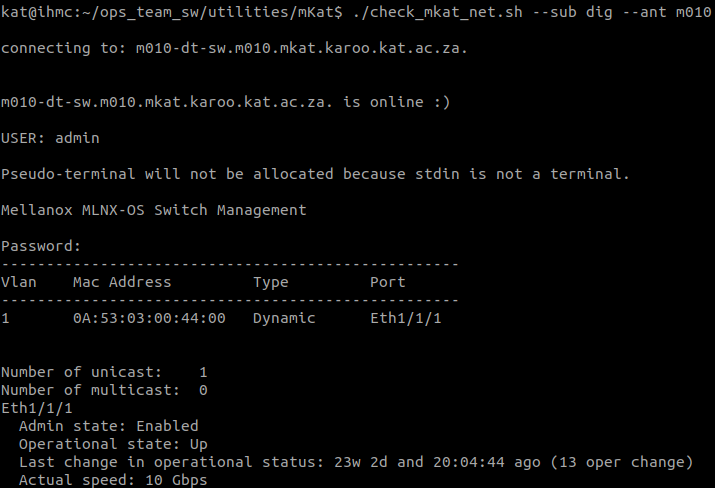
\includegraphics[scale=0.43]{Chapters/images/image75.png}
	
	%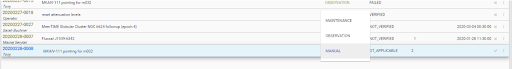
\includegraphics[resolution=100]{bur1.png}
	\caption{Output of \_net.sh script $-$ Digitiser status}
	\label{fig:image75}
\end{figure}


NOTE: L-band is connected to port: Eth1/1/1. If Eth1/1/1 is not up, power cycle the digitizer.

\subsection{ Using Observium to check the network status of nodes}
An alternative to monitoring the karoo telescope network is Observium. Observium uses SNMP (Simple Network Management Protocol) to monitor and manage network device status and traffic between them. Please use a “guest” account to only monitor the network nodes. 

Follow  the links below to monitor node groupings of the MeerKAT Telescope network
To login: \url{http://observium.kat.ac.za/}


Core Network: Link\_to\_site 

Receptor switches at the KAPB:\component{ M000-m031}  and  \component{m032-m064}

CBF Switches: Spines and Leafs

Digitizers: click the respective band on the last bulletin to load Observium. 
On Observium follow the routine below
Select the respective receptor data switch
The switch will be marked in red text if it is down
Then select the “Ports” button.
\begin{lstlisting}[style=DOS]
 
Links to the L-band digitizer are connected to Eth1/1/x
Links to the U-band digitizer are connected to Eth2/2/x
Links to the S-band digitizer are connected to Eth3/3/x
Links to the X-band digitizer are connected to Eth4/4/x 


\end{lstlisting}
U-Band        L-Band        S-Band        X-Band 


































